\chapter{Serverless computing} \label{cha:serverless}

This chapter serves as an introduction to serverless computing. Defining serverless computing succinctly can be difficult because of its relative immaturity. For example, the industry-standard NIST definitions of cloud computing \parencite{nist11definitions} have yet to catch up with the technology. Likewise the most recent ISO cloud computing vocabulary \parencite{iso14vocabulary} bears no mention of serverless computing. As a result boundaries between serverless and other areas of cloud computing areas are still somewhat blurred, and the terms seem to carry different meanings depending on the author and context. To complicate matters further, serverless computing has come to appear in two different but overlapping forms. A multilayered approach is therefore in order.

We approach the formidable task of defining serverless by first taking a brief look at the history and motivations behind utility computing. After that we'll introduce the basic tenets of serverless computing, distinguish between its two main approaches and see how it positions itself relative to other cloud service models. This is followed by a more technical look at the most recent serverless model, as well as its major providers, use cases, security issues and economic implications. The chapter closes with notes on the drawbacks and limitations of serverless, particularly from the point of view of web application backends.

This thesis' definition leans heavily on the industry-headed CNCF Serverless Working Group's effort to formalize and standardize serverless computing \parencite{cncf18serverlessWG}, as well as \citeauthor{robert2016serverlessarchitectures}'s (\citeyear{robert2016serverlessarchitectures}) seminal introduction to the topic and a number of recent survey articles \parencite[e.g.][]{baldini17currentTrends,van2017spec,fox17}. As a sidenote, although earliest uses of the term 'serverless' can be traced back to peer-to-peer and client-only solutions \parencite{fox17}, we're dismissing these references since the name has evolved into a completely different meaning in the current cloud computing context. As per \textcite{robert2016serverlessarchitectures}, first usages of the term referring to elastic cloud computing seem to have appeared at around 2012.

\section{Background} \label{sec:background}

Utility computing refers to a business model where computing resources, such as computation and storage, are commoditized and delivered as metered services similarly to physical public utilities such as water, electricity and telephony. Utilities are readily available to consumers at any time whenever required and billed per actual usage. In computing, this has come to mean on-demand access to highly scalable subscription-based IT resources. The availability of computing as an utility enables organizations to avoid investing heavily on building and maintaining complex IT infrastructure. \parencite{buyya09cloud}

This vision of utility computing can be traced all the way back to 1961, with the computing pioneer John McCarthy predicting that ``computation may someday be organized as a public utility'' \parencite{foster08cloudGrid}. Likewise in 1969 Leonard Kleinrock, one of the ARPANET chieft scientists, is quoted as saying, ``as of now, computer networks are still in their infancy, but as they grow up and become sophisticated, we will probably see the spread of ‘computer utilities’ which, like present electric and telephone utilities, will service individual homes and offices across the country'' \parencite{kleinrock03internet}. Creation of the Internet first facilitated weaving computer resources together into large-scale distributed systems. Onset by this discovery, multiple computing paradigms have been proposed and adopted over the years to take on the role of a ubiquitous computing utility, including cluster, grid, peer-to-peer (P2P) and services computing \parencite{buyya09cloud}. The latest paradigm, cloud computing, has in the past decade revolutionized the computer science horizon and got us closer to computing as an utility than ever \parencite{buyya2017manifesto}.

\textcite{sareen13cloudTypes} succinctly defines the cloud as ``a pool of virtualized computer resources''. \textcite{foster08cloudGrid} present a more thorough definition of cloud computing as ``a large-scale distributed computing paradigm that is driven by economies of scale, in which a pool of abstracted, virtualized, dynamically-scalable, managed computing power, storage, platforms, and services are delivered on demand to external customers over the Internet''. Cloud computing builds on the earlier paradigm of grid computing, and relies on grid computing as its backbone and infrastructure. Compared to infrastructure-based grid computing, cloud computing focuses on more abstract resources and services. \textcite{buyya2017manifesto} also note that cloud computing differs from grid computing in that it promises virtually unlimited computational resources on demand.

The first cloud providers were born out of huge corporations offering their surplus computing resources as a service in order to offset expenses and improve utilization rates. Having set up global infrastructure to handle peak demand, a large part of the resources were left under-utilized at times of average demand. The providers are able to offer these surplus resources at attractive prices due to the large scale of their operations, benefiting from economies of scale. To address consumers' concerns about outages and other risks, cloud providers guarantee a certain level of service delivery through Service Level Agreements (SLA) that are negotiated between providers and consumers. \parencite{youseff08cloudOntology}

The key technology that enables cloud providers to transparently handle consumers' requests without impairing their own processing needs is \textit{virtualization}. Virtualization is one of the main components behind cloud computing and one of the factors setting it apart from grid computing. \textcite{sareen13cloudTypes} defines virtualization as using computer resources to imitate other computer resources or whole computers. This enables the abstraction of the underlying physical resources as a set of multiple logical virtual machines (VM). Virtualization has three characteristics that make it ideal for cloud computing: 1) \textit{partitioning} supports running many applications and operating systems in a single physical system; 2) \textit{isolation} ensures boundaries between the host physical system and virtual containers; 3) \textit{encapsulation} enables packaging virtual machines as complete entities to prevent applications from interfering with each other.

Virtual machines manage to provide strong security guarantees by isolation, i.e., by allocating each VM its own set of resources with minimal sharing between the host system. Minimal sharing however translates into high memory and storage requirements as each virtual machine requires a full OS image in addition to the actual application files. A virtual machine also has to go through the standard OS boot process on startup, resulting in launch times measured in minutes. Rapid innovation in the cloud market and virtualization technologies has recently lead to an alternative, more lightweight \textit{container}-based solution. Container applications share a kernel with the host, resulting in significantly smaller deployments and fast launch times ranging from less than a second to a few seconds. Due to resource sharing a single host is capable of hosting hundreds of containers simultaneously. Differences in resource sharing between VM- and container-based deployment is illustrated in figure \ref{fig:vmVsContainer}. As a downside containers lack the VM's strong isolation guarantee and the ability to run a different OS per deployment. On the other hand, containers provide isolation via namespaces, so processes inside containers are still isolated from each other as well as the host. \textit{Containerization} has emerged as a common practice of packaging applications and related dependencies into standardized container images to ease development efficiency and interoperability. \parencite{pahl15containerization}

\begin{figure}[h]
  \centering
  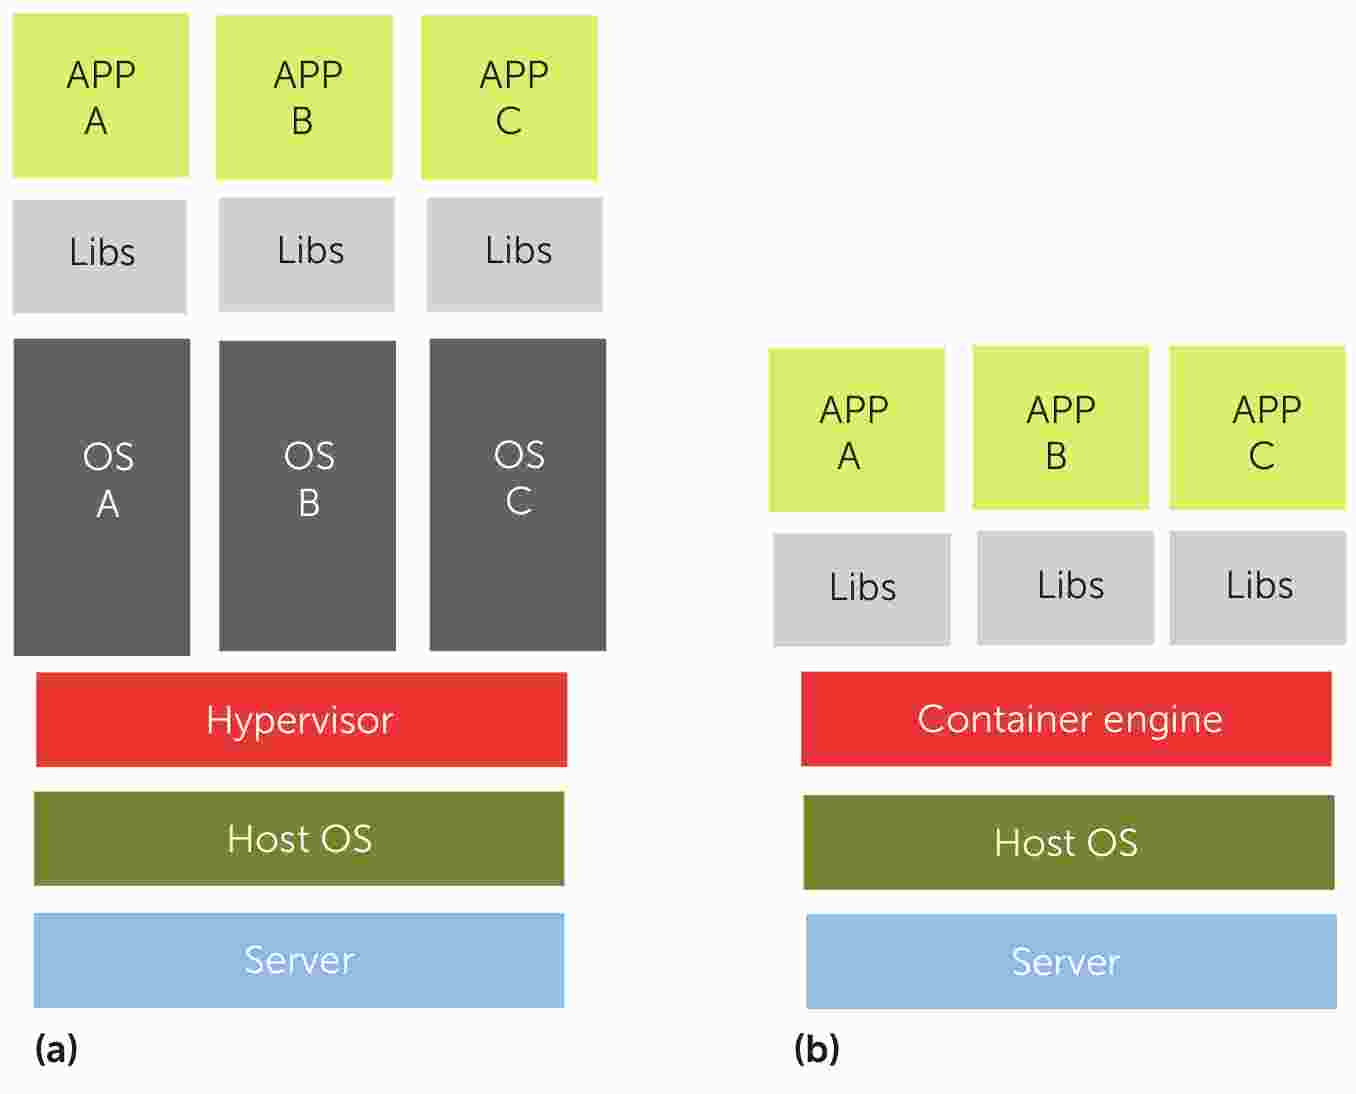
\includegraphics[width=0.8\textwidth]{bernstein14-vm-vs-container.jpg}
  \caption{Comparison of a) virtual machine- and b) container-based deployments \parencite{bernstein14containers}}
  \label{fig:vmVsContainer}
\end{figure}

Cloud computing is by now a well-established paradigm that enables organizations to flexibly deploy a wide variety of software systems over a pool of externally managed computing resources. Both major IT companies and startups see migrating on-premise legacy systems to the cloud as an opportunistic business strategy for gaining competetive advantage. Cost savings, scalability, reliability and efficient utilization of resources as well as flexibility are identified as key drivers for migrating applications to the cloud \parencite{jamshidi13cloudmigrationreview}. However, although the state-of-the-art in cloud computing has advanced significantly over the past decade, several challenges remain.

One of the open issues in cloud computing concerns pricing models. In the current cloud service models pricing typically follows the ``per instance per hour'' model; that is, the consumer is charged for the duration that an application is hosted on a VM or a container \parencite{varghese18next}. The flaw in this model is that idle time is not taken into account. Whether the application was used or not bears no effect: the consumer ends up paying for the whole hour even if the application was actually performing computation for mere seconds. This makes sense from the provider's point of view, since for the duration billed, the instance is provisioned and dedicated solely to hosting the consumer's application. However, paying for idle time is of course undesirable for the consumer, and the problem is made worse in case of applications with fluctuating and unpredictable workloads.

Continuously hosting non-executing applications is problematic on the provider side as well as it leads to under-utilization. Just as consumers end up paying for essentially nothing, providers end up provisioning and tying up resources to do essentially nothing. Fundamentally the problem of under-utilization boils down to elasticity and resource management. The current cloud computing models are incapable of automatically scaling up and down to meet current demand while at the same time maintaining their stringent Quality-of-Service (QoS) expectations \parencite{buyya2017manifesto}. Lacking automatic scaling mechanisms, cloud consumers are left to make capacity decisions on their own accord, and as \textcite{robert2016serverlessarchitectures} notes, consumers typically err on the side of caution and over-provision. This in turn leads to inefficiencies and under-utilization as described above.

The problem of low utilization rates in data centers is particularly relevant in the current energy-constrained environment. ICT in general consumes close to 10\% of all electricity world-wide, with the CO$_2$ impact comparable to air travel \parencite{buyya2017manifesto}. It's estimated that in 2010 data centers accounted for 1-2\% of global energy usage, with data center carbon emissions growing faster than the annual global footprint as well as the footprint of other ICT subcategories. While data centers are improving in energy efficiency, so is the demand for computing services with both the magnitude of data produced and complexity of software increasing. Operational factors such as excessive redundancy also affect data center energy efficiency heavily. A survey of Google data centers -- considered to represent the higher end of utilization -- revealed utilization of 60\% or less 95\% of the time and 30\% or less half of the time. Another analysis found that data centers spend on average only 6\% to 12\% of the electricity powering servers that do computation, with the rest used to keep servers idling for redundancy. \parencite{horner16powerusage}

Cloud computing, having ``revolutionized the computer science horizon and enabled the emergence of computing as the fifth utility'' \parencite{buyya2017manifesto}, will face considerable new requirements in the coming decade. It's predicted that by 2020 over 20 billion sensor-rich devices like phones and wearables will be connected to the Internet generating trillions of gigabytes of data. \textcite{varghese18next} argue that increasing volumes of data pose significant networking and computing challenges that cannot be met by existing cloud infrastructure, and that adding more centralized cloud data centers will not be enough to address the problem. The authors instead call for new computing models beyond conventional cloud computing, one of which is serverless computing.

\section{Defining serverless} \label{sec:definingServerless}

\textcite{van2017spec} define serverless computing as ``a form of cloud computing that allows users to run event-driven and granularly billed applications, without having to address the operational logic''. The definition breaks down into three key characteristics: \begin{enumerate}
  \item Event-driven: interactions with serverless applications are designed to be short-lived, allowing the infrastructure to deploy serverless applications to respond to events, so only when needed.
  \item Granular billing: the user of a serverless model is charged only when the application is actually executing.
  \item (Almost) no operational logic: operational logic, such as resource management and autoscaling, is delegated to the infrastructure, making those concerns of the infrastructure operator.
\end{enumerate}

Fundamentally serverless computing is about building and running back-end code that does not require server management or long-lived server applications. The term itself can seem disingenuous, since serverless computing obviously still involves servers. The name -- coined by industry -- instead carries the meaning that operational concerns are fully managed by the cloud service provider. As tasks such as provisioning, maintenance and capacity planning are outsourced to the serverless platform, developers are left to focus on application logic and more high-level properties such as control, cost and flexibility. For the cloud customer this provides an abstraction where computation is disconnected from the infrastructure it runs on. \parencite{robert2016serverlessarchitectures,cncf18serverlessWG}

\begin{figure}[h]
  \centering
  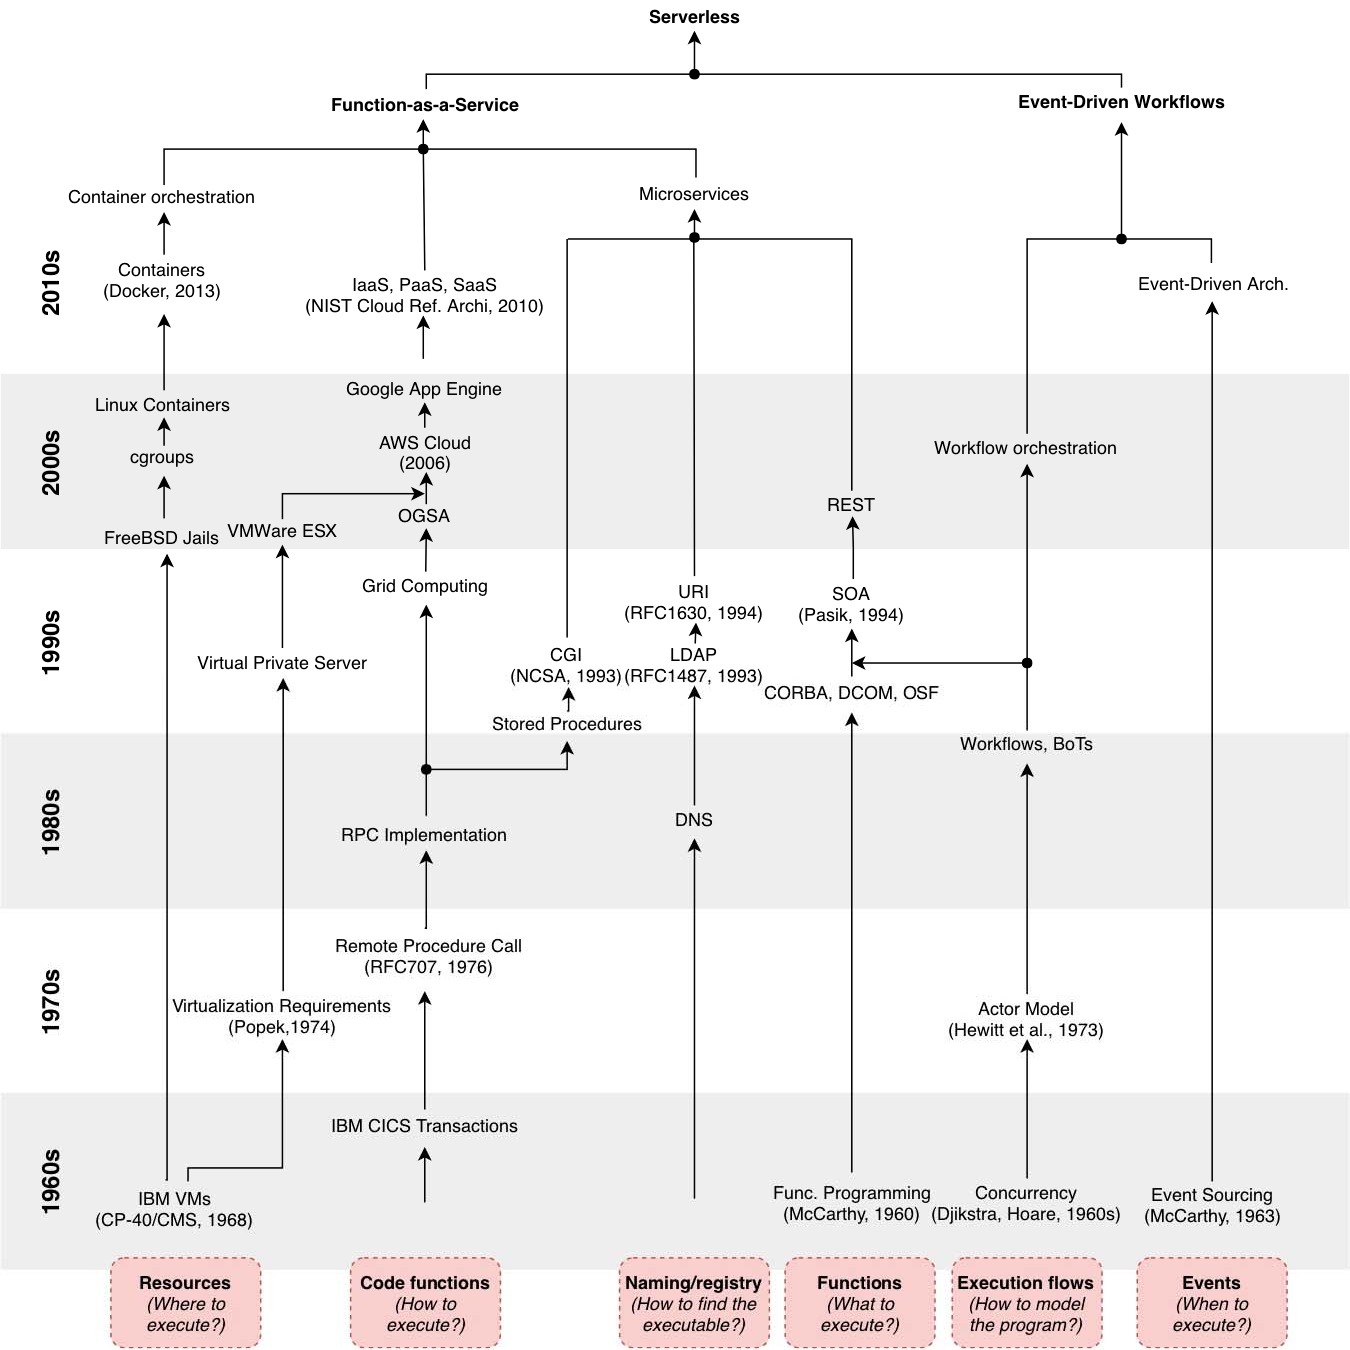
\includegraphics[width=0.9\textwidth]{eyk18-serverless-lineage.png}
  \caption{A history of computer science concepts leading to serverless computing \parencite{van18fromPAAStoPresent}}
  \label{fig:serverlessLineage}
\end{figure}

Serverless platforms position themselves as the next step in the evolution of cloud computing architectures \parencite{baldini17currentTrends}. \textcite{van18fromPAAStoPresent} trace the computing technologies that lead to the emergence of serverless computing in figure \ref{fig:serverlessLineage}. First of all the rapid progress in systems infrastructure technologies, specifically virtualization and containerization as described in section \ref{sec:background}, made serverless platforms technically feasible. Secondly, software architecture trends transitioning from ``relatively large, monolithic applications, to smaller or more structured applications with smaller executions units'' \parencite{van2017spec} paved the way for the serverless concept of functions as computation. \textcite{van18fromPAAStoPresent} see serverless computing continuing this trend of service specialization and abstraction, preceded by Service-Oriented Architecture and later by microservices. Finally the transition from synchronous systems to concurrent, event-driven distributed systems laid the groundwork for the serverless execution model: as per \textcite{mcgrath17implement}, serverless computing ``is a partial realization of an event-driven ideal, in which applications are defined by actions and the events that trigger them''.

\subsection{Backend-as-a-Service and Function-as-a-Service} \label{subsec:faasbaas}

Serverless computing has in effect come to encompass two distinct cloud computing models: Backend-as-a-Service (BaaS) as well as Function-as-a-Service (FaaS). The two serverless models, while different in operation as explained below, are grouped under the same serverless umbrella since they deliver the same main benefits: zero server maintenance overhead and elimination of idle costs. \parencite{cncf18serverlessWG}

Backend-as-a-Service refers to an architecture where an application's server-side logic is replaced with external, fully managed cloud services that carry out various tasks like authentication or database access \parencite{buyya2017manifesto}. The model is typically utilized in the mobile space to avoid having to manually set up and maintain server resources for the more narrow back-end requirements of a mobile application. In the mobile context this form of serverless computing is also referred to as Mobile-Backend-as-a-Service or MBaaS \parencite{sareen13cloudTypes}. An application's core business logic is implemented client-side and integrated tightly with third party remote application services. Since these API-based BaaS services are managed transparently by the cloud service provider, the model appears to the developer as serverless.

Function-as-a-Service is defined in a nutshell as ``a style of cloud computing where you write code and define the events that should cause the code to execute and leave it to the cloud to take care of the rest'' \parencite{gannon17cloudNative}. In the FaaS architecture an application's business logic is still located server-side. The crucial difference is that instead of self-managed server resources, developers upload small units of code to a FaaS platform that executes the code in short-lived, stateless compute containers in response to events \parencite{robert2016serverlessarchitectures}. The model appears serverless in the sense that the developer has no control over the resources on which the back-end code runs. \textcite{albuquerque17faaspaas} note that the BaaS model of locating business logic on the client side carries with it some complications, namely difficulties in updating and deploying new features as well as reverse engineering risks. FaaS circumvents these problems by retaining business logic server-side.

Out of the two serverless models FaaS is a more recent development: the first commercial FaaS platform, AWS Lambda, was introduced in November 2014 \parencite{awslambda0218}.
FaaS is also the model with significant differences to traditional web application architecture \parencite{robert2016serverlessarchitectures}. These differences and their implications are further illustrated in section \ref{sec:processingModel}. As the more novel architecture, FaaS is especially relevant to the research questions in hand and is thus paid more attention to in the remainder of this thesis.

Another perspective on the difference between the two serverless models is to view BaaS as a more tailored, vendor-specific approach to FaaS \parencite{van2017spec}. Whereas BaaS-type services function as built-in components for many common use cases such as user management and data storage, a FaaS platform allows developers to implement more customized functionality. BaaS plays an important role in serverless architectures as it will often be the supporting infrastructure (e.g. in form of data storage) to the stateless FaaS functions \parencite{cncf18serverlessWG}. Conversely, in case of otherwise BaaS-based applications there's likely still a need for custom server-side functionality; FaaS functions may be a good solution for this \parencite{robert2016serverlessarchitectures}. Serverless applications can utilize both models simultaneously, with BaaS platforms generating events that trigger FaaS functions, and FaaS functions acting as a 'glue component' between various third party BaaS components. \textcite{robert2016serverlessarchitectures} also notes convergence in the space, giving the example of the user managemement provider Auth0 starting initially with a BaaS-style offering but later entering the FaaS space with a 'Auth0 Webtask' service.

It's worth noting that not all authors follow this taxonomy of FaaS and BaaS as the two subcategories of a more abstract serverless model. \textcite{baldini17currentTrends} explicitly raise the question on whether serverless is limited to FaaS or broader in scope, identifying the boundaries of serverless as an open question. Some sources \parencite[][among others]{hendrickson16openlambda,mcgrath17implement,varghese18next} seem to strictly equate serverless with FaaS, using the terms synonymously. Considering however that the term 'serverless' predates the first FaaS platforms by a couple of years \parencite{robert2016serverlessarchitectures}, it seems sensible to at least make a distinction between serverless and FaaS. In this thesis we'll stick to the \textcite{cncf18serverlessWG} definition as outlined above.

\section{Comparison to other cloud computing models} \label{sec:comparisonCloud}

% As serverless is gaining popularity the boundaries between different types of ”as-a-Service” may be disappearing (see Figure 9). One could imagine that developers not only write code but also declare how they want the code to run - as FaaS orMBaaS or PaaS - and can change as needs change. In the future the main distinction may be between caring about server (server-aware) and not caring about server details (server-less). PaaS is in the middle; it makes it very easy to deploy code but developers still need to know about servers and be aware of scaling strategies, such as how many instances to run. \parencite{baldini17currentTrends}

Another approach to defining serverless is to compare it with other cloud service models. The commonly used NIST definition \parencite{nist11definitions} divides cloud offerings into three categories: Infrastructure-as-a-Service (IaaS), Platform-as-a-Service (PaaS) and Software-as-a-Service (SaaS), in increasing order of infrastructure abstraction \parencite{nist11definitions}. As per \textcite{buyya2017manifesto}, SaaS allows users to access complete applications hosted in the cloud, PaaS offers a framework for creation and development of more tailored cloud applications, and finally IaaS offers access to computing resources in form of leased VMs and storage space. On this spectrum serverless computing positions itself in the space between PaaS and SaaS, as illustrated in figure \ref{fig:degreeOfAutomation} \parencite{baldini17currentTrends}. Figure \ref{fig:cloudSpectrum} illustrates how the two serverless models relate, with the cloud provider taking over a larger share of operational logic in BaaS. \textcite{van2017spec} note that there's some overlap and give examples of non-serverless products in both the PaaS and SaaS worlds that nonetheless exhibit the main serverless characteristics defined in section \ref{sec:definingServerless}.

\begin{figure}[h]
  \centering
  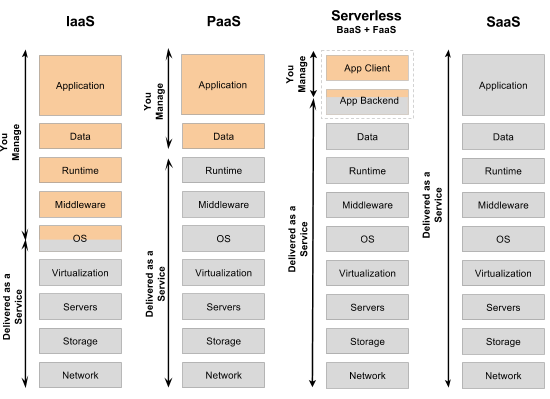
\includegraphics[width=0.9\textwidth]{specify-io-cloud-comparison.png}
  \caption{Degree of automation when using serverless \parencite{wolf16serverless}}
  \label{fig:degreeOfAutomation}
\end{figure}

\begin{figure}[h]
  \centering
  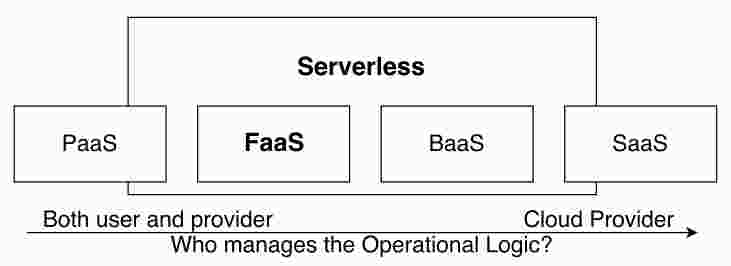
\includegraphics[width=0.8\textwidth]{eyk17-cloud-comparison.jpg}
  \caption{Serverless and FaaS vs. PaaS and SaaS \parencite{van2017spec}}
  \label{fig:cloudSpectrum}
\end{figure}

Since the gap between PaaS and FaaS can be quite subtle it warrants further consideration. Indeed some sources \parencite[e.g.][]{adzic2017serverless} refer to FaaS as a new generation of PaaS offerings. Both models provide a high-level and elastic computing platform on which to implement custom business logic. There are however a number of substantial differences between the two models, which ultimately boil down to PaaS being an instance-based model with multiple server processes running on always-on server instances, as opposed to the on-demand resource allocation of FaaS. Put another way, ``most PaaS applications are not geared towards bringing entire applications up and down for every request, whereas FaaS platforms do exactly this'' \parencite{robert2016serverlessarchitectures}.

\textcite{albuquerque17faaspaas} derive a number of specific differences between PaaS and FaaS in their comparative analysis. First of all the units of deployment vary: PaaS applications are deployed as services, compared to the more granular function-based deployment of FaaS. Second, PaaS instances are always running whereas serverless workloads are executed on-demand. Third, PaaS platforms, although supporting auto-scaling to some extent, require the developer to explicitly manage the scaling workflow and number of minimum instances. FaaS on the other hand scales transparently and on-demand without any need for resource pre-allocation. Perhaps the most important distinction lies in billing: PaaS is billed by instantiated resources whether they're used or not, whereas FaaS is billed per-event only for the execution duration. The analysis concludes that PaaS is well suited for predictable or constant workloads with long or variable per-request execution times; FaaS in turn provides better cost benefit for unpredictable or seasonal workloads with short per-request execution times. It's also to be noted that PaaS doesn't suffer from limits on execution duration and many other restrictions of FaaS as described in section \ref{sec:limitations}.

\section{Serverless processing model} \label{sec:processingModel}

The \textcite{cncf18serverlessWG} whitepaper divides a generalized serverless solution into four constituents, as illustrated in figure \ref{fig:processingModel}:

\begin{itemize}
  \item Event sources - trigger or stream events into one or more function instances.
  \item Function instances - a single function/microservice, that can be scaled with demand.
  \item FaaS Controller- deploy, control and monitor function instances and their sources.
  \item Platform services - general cluster or cloud services (BaaS) used by the FaaS solution.
\end{itemize}

\begin{figure}[h]
  \centering
  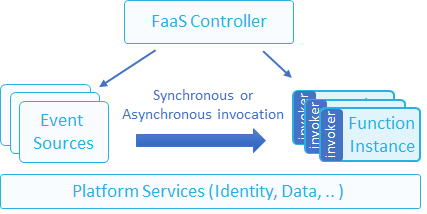
\includegraphics[width=0.8\textwidth]{cncf18-serverless-processing-model.png}
  \caption{Serverless processing model \parencite{cncf18serverlessWG}}
  \label{fig:processingModel}
\end{figure}

Interrelation of the various parts is further demonstrated with an example of a typical serverless development workflow. First, the developer selects a runtime environment (e.g. Python 3.6), writes a piece of code and uploads it on a FaaS platform where the code is published as a serverless function. The developer then maps one or more event sources to trigger the function, with event sources ranging from HTTP calls to database changes and messaging services. Now when any of the specified events occurs, the FaaS ontroller spins up a container, loads up the function along with its dependencies and executes the code. The function code typically contains API calls to external BaaS resources to handle data storage and other integrations. When there are multiple events to respond to simultaneously, more copies of the same function are run in parallel. Serverless functions thus scale precisely with the size of the workload, down to the individual request. After execution the container is torn down. Later the developer is billed according to the measured execution time, typically in 100 millisecond increments. \parencite{awslambda0218}

At the heart of serverless architecture is the concept of a function (also \textit{lambda function} or \textit{cloud function}). A function represents a piece of business logic executed in response to specified events. Functions are the fundamental building block from which to compose serverless applications. A function is defined as a small, stateless, short-lived, on-demand service with a single functional responsibility \parencite{van2017spec}. As discussed in section \ref{sec:background}, the technology underlying cloud computing has evolved from individual servers to virtual machines and containers. \textcite{hendrickson16openlambda} see the serverless function model as the logical conclusion of this evolution towards more sharing between applications (figure \ref{fig:evolutionOfSharing}).

\begin{figure}[h]
  \centering
  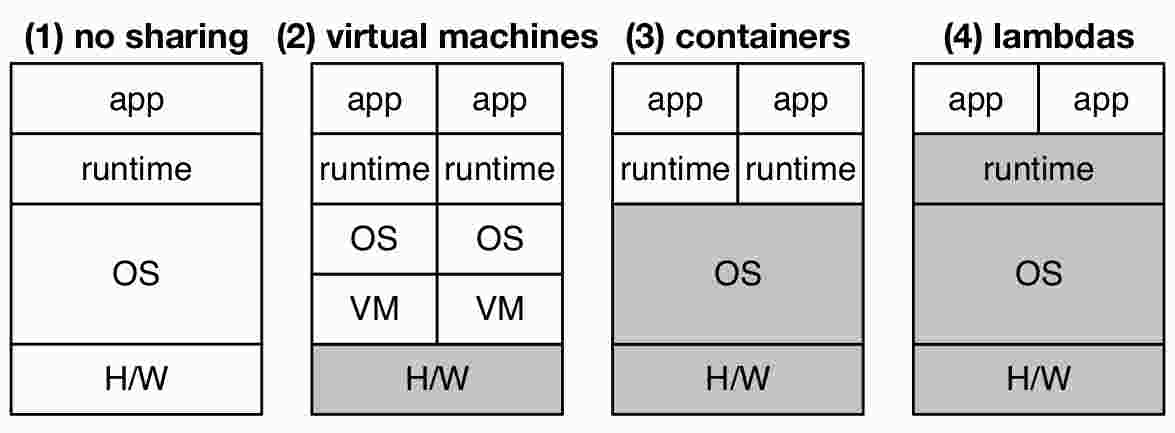
\includegraphics[width=0.8\textwidth]{hendrickson16-evolution-of-sharing.jpg}
  \caption{Evolution of sharing -- gray layers are shared \parencite{hendrickson16openlambda}}
  \label{fig:evolutionOfSharing}
\end{figure}

Being stateless and short-lived, serverless functions have fundamentally limited expressiveness compared to a conventional PaaS-hosted application. This is a direct result of being built to maximise scalability. A FaaS platform will need to execute the arbitrary code in a function in response to any number of events, without explicitly specifying resources required for the operation \parencite{buyya2017manifesto}. To make this possible, FaaS platforms pose restrictions on what functions can do and how long they can operate. Statelessness here means that a function loses all local state after termination; none of the local state created during invocation will necessarily be available during subsequent invocations of the same function. This is where BaaS services come in, with external stateful services such as key-value stores, databases and file or blob storages providing a persistence layer. In addition to statelessness, FaaS platforms limit a funtion's execution duration and resource usage: AWS Lambda for example has a maximum execution duration of 15 minutes and a maximum memory allocation of 3008 MB \parencite{awslambda0218}.

FaaS event sources can be divided into two categories, synchronous and asynchronous. The first category follows a typical request-response flow: a client issues a request and blocks while waiting for a response. Synchronous event sources include HTTP and RPC calls which can be used to implement a REST API, a command line client or any other service requiring immediate feedback. Asynchronous event sources on the other hand result in non-blocking function execution, and they're typically used to implement background workers, scheduled event handlers and queue workers. Asynchronous event sources include message queues, publish-subscribe systems, database or file storage change feeds and CRON jobs among others. The details and metadata of the triggering event are passed to the function as an input parameter, with exact implementation varying per event type and provider. In case of a HTTP call, for example, the event object might include the request path, headers, body and query parameters. A function instance is also commonly supplied a context object, which in turn contains runtime information and other general properties that span multiple function invocations. Function name, version, memory limit and remaining execution time are examples of typical context variables. FaaS platforms also usually allow users to set environment variables which function instances can access through the context object -- useful for handling security keys and tokens. As for output, functions can either directly return a value (in case of synchronous invocation) or either trigger the next execution phase in a workflow or simply log the result (in case of asynchronous invocation). An example function handler is presented in listing \ref{lst:handlerExample}. In addition to publishing and executing serverless functions, FaaS platforms also typically provide auxiliary capabilities such as monitoring, statistics, versioning and logging. \parencite{cncf18serverlessWG}

\renewcommand\thelstlisting{\arabic{lstlisting}}
\setcounter{lstlisting}{0}
\begin{lstlisting}[language=Python,caption=Example FaaS handler,captionpos=b,label=lst:handlerExample,showstringspaces=false,belowskip=2em,frame=tb,aboveskip=2em]
  def main(event, context):
      return {"payload": "Hello, " + event.name}
\end{lstlisting}

As mentioned in section \ref{sec:definingServerless}, serverless is \textit{almost} but not completely devoid of operational management. In case of serverless functions, this qualification means that parameters such as memory reservation size, maximum parallelism and execution time are still left for the user to configure. Whereas the latter parameters are mainly used as safeguards to control costs, memory reservation size has important implications regarding execution efficiency \parencite{lloydserverless}. There are however tools available to determine the optimal memory reservation size per given workload. Also some platforms automatically reserve the required amount of memory without pre-allocation \parencite{microsoft18azureFunctions}.

% \textcite{fox17} present a useful short definition of a FaaS platform like Lambda as a cloud-native platform for short-running, stateless computation and event-driven applications which scales up and down instantly and automatically and charges for actual usage at a millisecond granularity.

Even with the restrictions on a serverless function's capabilities, implementing a FaaS platform is a difficult problem. From the customer's point of view the platform has to be as fast as possible in both spin-up and execution time, as well as scale indefinitely and transparently. The provider on the other hand seeks maximum resource utilization at minimal costs while avoiding violating the consumer's QoS expectations. Given that these goals are in conflict with each other, the task of resource allocation and scheduling bears crucial importance \parencite{reza17controller}. A FaaS platform must also safely and efficiently isolate functions from each other, and make low-latency decisions at the load balancer-level while considering session, code, and data locality \parencite{hendrickson16openlambda}.

\section{Use cases} \label{sec:useCases}

Serverless computing has been utilized to support a wide range of applications. \textcite{baldini17currentTrends} note that from a cost perspective, the model is particularly fitting for bursty, CPU-intensive and granular workloads, as well as applications with sudden surges of popularity such as ticket sales. Serverless is less suitable for I/O-bound applications where a large period of time is spent waiting for user input or networking, since the paid-for compute resources go unused. In the industry, serverless is gaining traction primarily in three areas: Internet-of-Things (IoT) applications with sporadic processing needs, web applications with light-weight backend tasks, and as glue code between other cloud computing services \parencite{spillner18faaster}.

A number of real-world and experimental use cases exists in literature. \textcite{adzic2017serverless} present two industrial case studies implementing mind-mapping and social networking web applications in serverless architectures, resulting in decreased hosting costs. \textcite{mcgrath16cloudEventParadigms} describe a serverless media management system that easily and performantly solves a large-scale image resizing task. \textcite{fouladi2017encoding} present a serverless video-processing framework. \textcite{yan16chatbot,lehva18chatbot} both implement serverless chatbots, reaching gains in cost and management efficiency. \textcite{ast17webcomponent} describe an approach to building truly self-contained serverless web components.

In the domain of high-performance and scientific computing, \textcite{jonas17occupy} suggest that ``a serverless execution model with stateless functions can enable radically-simpler, fundamentally elastic, and more user-friendly distributed data processing systems''. \textcite{malawski17executescientific} experiment with running scientific workflows on a FaaS platform and find the approach easy to use and highly promising, noting however that not all workloads are suitable due to execution time limits. \textcite{spillner18faaster} similarly find that ``in many domains of scientific and high-performance computing, solutions can be engineered based on simple functions which are executed on commercially offered or self-hosted FaaS platforms''. \textcite{ishakian17neural} evaluate the suitability of a serverless computing environment for the inferencing of large neural network models. \textcite{petrenko17nasa} present a NASA data exploration tool running on a FaaS platform.

The novel paradigms of edge and fog computing are identified as particularly strong drivers for serverless computing \parencite{fox17}. These models seek to include the edge of the network in the cloud computing ecosystem to bring processing closer to the data source and thus reduce latencies between users and servers \parencite{buyya2017manifesto}. The need for more localized data processing stems from the growth of mobile and IoT devices as well as the demand for more data-intensive tasks such as mobile video streaming. Bringing computation to the edge of the network addresses this inreasing demand by avoiding the bottlenecks of centralized servers and latencies introduced by sending and retrieving heavy payloads from and to the cloud \parencite{baresi17edgecomputing}. \textcite{nastic17analyticsedge} explain how the increasing growth of IoT devices has lead to ``an abundance of geographically dispersed computing infrastructure and edge resources that remain largely underused for data analytics applications'' and how ``at the same time, the value of data becomes effectively lost at the edge by remaining inaccessible to the more powerful data analytics in the cloud due to networking costs, latency issues, and limited interoperability between edge devices''.

Despite the potential efficiencies gained, hosting and scaling applications at the edge of the network remains problematic with edge/fog computing environments suffering from high complexity, labor-intensive lifecycle management and ultimately high cost \parencite{glikson17devicelessedge}. Simply adopting the conventional cloud technologies of virtual machines and containers at the edge is not possible since the underlying resource pool at the edge is by nature highly distributed, heterogeneous and resource-constrained \parencite{baresi17edgecomputing}. Serverless computing, with its inherent scalability and abstraction of infrastructure, is recognized by multiple authors as a promising approach to address these issues. \textcite{nastic17analyticsedge} present a high-level architecture for a serverless edge data analytics platform. \textcite{baresi17edgecomputing} propose a serverless edge architecture and use it to implement a low-latency high-throughput mobile augmented reality application. \textcite{glikson17devicelessedge} likewise propose a novel approach that extends the serverless platform to the edge of the network, enabling IoT and Edge devices to be seamlessly integrated as application execution infrastructure. In addition, \textcite{van2017spec} lay out a vision of a vendor-agnostic FaaS layer that would allow an application to be deployed in hybrid clouds, with some functions deployed in an on-premise cluster, some in the public cloud and some running in the sensors at the edge of the cloud.

\section{Service providers} \label{sec:providers}

\textcite{lynn2017preliminary} provide an overview and multi-level feature analysis of the various enterprise serverless computing platforms. The authors identified seven different commercial platforms: AWS Lambda, Google Cloud Functions, Microsoft Azure Functions, IBM Bluemix OpenWhisk, Iron.io Ironworker, Auth0 Webtask, and Galactic Fog Gestal Laser. All the platforms provide roughly the same basic functionality, with differences in the available integrations, event sources and resource limits. The most commonly supported runtime languages are Javascript followed by Python, with secondary support for Java, C\#, Go, Ruby, Swift and others. The serverless platforms of the big cloud service providers, Amazon, Google, Microsoft and IBM, benefit from tight integration with their respective cloud ecosystems. The study finds that AWS Lambda, the oldest commercial serverless platform, has emerged as a \textit{de facto} base platform for research on enterprise serverless cloud computing. AWS Lambda has also the most cited high profile use cases ranging from video transcoding at Netflix to data analysis at Major League Baseball Advanced Media. Google Cloud Functions remains in beta stage at the time of writing, and has limited functionality but is expected to grow in future versions \parencite{google18cloudFunctions}. The architecture of OpenWhisk is shown in figure \ref{fig:openwhisk} as an example of a real-world FaaS platform. Besides the commercial offerings, a number of self-hosted open-source FaaS platforms have emerged: the \textcite{cncf18serverlessWG} whitepaper mentions fission.io, Fn Project, kubeless, microcule, Nuclio, OpenFaaS and riff among others. The core of the commercial IBM OpenWhisk is also available as an Apache open-source project \parencite{ibm18cloudFunctions}. In addition, research-oriented FaaS platforms have been presented in literature, including OpenLambda \parencite{hendrickson16openlambda} and Snafu \parencite{spillner17snafu}.

\begin{figure}[h]
  \centering
  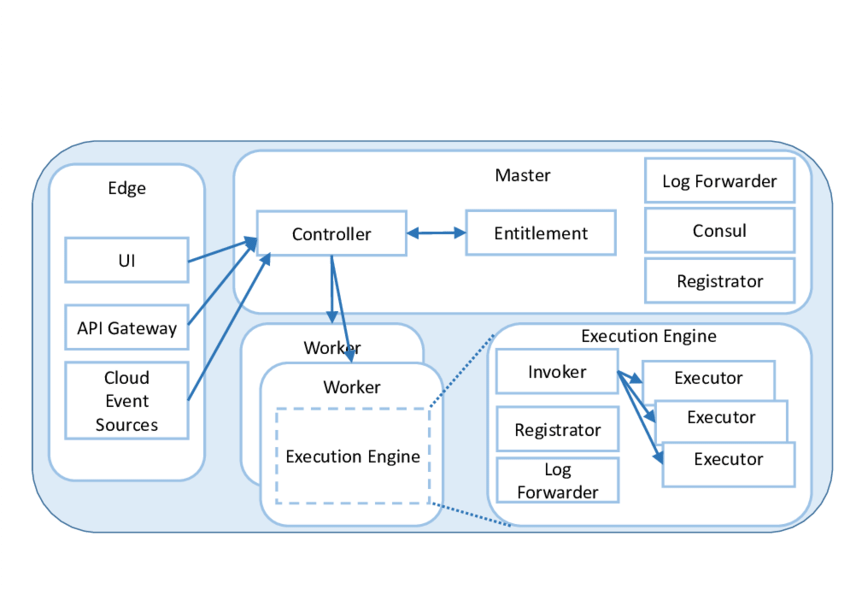
\includegraphics[width=0.9\textwidth]{baldini17-openwhisk-architecture.png}
  \caption{IBM OpenWhisk architecture \parencite{baldini17currentTrends}}
  \label{fig:openwhisk}
\end{figure}

The big four FaaS platforms are compared in a recent benchmark by \textcite{malawski18benchmark}. Each platform requires the user to configure a function's memory size allocation -- apart from Azure Functions which allocate memory automatically. Available memory sizes range from 128 to 2048MB, with the per-invocation cost increasing in proportion to memory size. Measuring the execution time of CPU-intensive workloads with varying function sizes, the authors observe interesting differences in resource allocation between the different providers. AWS Lambda performs fairly consistently with CPU allocation increasing together with memory size as per the documentation. Google Cloud Functions instead behave less predictably with the smallest 128MB functions occasionally reaching the performance of the largest 2048MB functions. The authors suggest this results from an optimization in container reuse, since reusing already spawned faster instances is cheaper than spinning up new smaller instances. Azure Functions show on average slower execution times, which the authors attribute to the underlying Windows OS and virtualization layer. On both Azure Functions and IBM Bluemix performance does not depend on function size.

A consequence of the high abstraction level of serverless computing is that the commercial FaaS platforms are essentially black boxes, with little guarantee about underlying resources. There are however efforts to gain insight into the platforms via reverse engineering. \textcite{wang18peekingbehindcurtains} present the ``largest measurement study to date, launching more than 50,000 function instances across these three services, in order to characterize their architectures, performance, and resource management efficiency''. One of the findings is that all service providers exhibit a variety of VMs as hosts, which may cause inconsistent function performance. The study also reveals differences on how serverless platforms allocate functions to host VMs. Both AWS Lambda and Azure Functions scale function instances on the same VM, which results in resource contention as each function gets a smaller share of the network and I/O resources. Among the compared platforms, AWS Lambda achieved the best scalability and lowest start-up latency for new function instances.

\section{Security} \label{sec:security}

Similarly to PaaS, serverless architecture addresses most of the OS-level security concerns by pushing infrastructure management to the provider. Instead of users maintaining their own servers, security-related tasks like vulnerability patching, firewall configuration and intrusion detection are centralized with the benefit of a reduced attack surface. On the provider side the key issue becomes guaranteeing isolation between functions, as arbitrary code from many users is running on the same shared resources \parencite{mcgrath17implement}. Since strong isolation has the downside of longer container startup times, the problem becomes finding an ideal trade-off between security and performance. \parencite{van2017spec}

In case of the BaaS model, the main security implication is greater dependency to third party services \parencite{segal18risks}. Each BaaS component represents a potential point of compromise, so it becomes important to secure communications, validate inputs and outputs and minimize and anonymize the data sent to the service. \textcite{robert2016serverlessarchitectures} also notes that since BaaS components are used directly by the client, there's no protective server-side application in the middle which requires significant care in designing the client application.

The FaaS model has a number of advantages when it comes to security. First, FaaS applications are more resilient towards Denial of Service (DoS) attacks due to the platform's near limitless scalability -- although such an attack can still inflate the monthly bill and inflict unwanted costs. Second, compromised servers are less of an issue in FaaS since functions run in short-lived containers that are repeatedly destroyed and reset. Overall, as put by \textcite{wagner16resilient}, ``there is a much smaller attack surface when executing on a platform that does not allow you to open ports, run multiple applications, and that is not online all of the time''. On the other hand application-level vulnerabilities remain as much of an issue in FaaS as in conventional cloud platforms. The architecture has no inherent protection against SQL injection or XSS and CSRF attacks, so existing mitigation techniques are still necessary. Vulnerabilities in application dependencies are another potential threat, since open-source libraries often make up the majority of the code in actual deployed functions. Also, the ease and low cost of deploying a high number of functions, while good for productivity, requires new approaches to security monitoring. With each function expanding the application's attack surface it's important to keep track of ownership and allocate a function only the minimum privileges needed to perform the intended logic. Managing secure configuration per each funtion can become cumbersome with fine-grained applications consisting of dozens or hundreds of functions. \parencite{podjarny17security}

A study by the security company PureSec lists a number of prominent security risks specific to serverless architectures \parencite{segal18risks}. One potential risk concerns event data injection, i.e. functions inadvertently executing malicious input injected among the event payload. Since serverless functions accept a rich set of event sources and payloads in various message formats, there are many opportunities for this kind of injection. Another risk listed in the study is execution flow manipulation. Serverless architectures are particularly vulnerable to flow manipulation as applications typically consist of many discrete functions chained together in a specific order. Application design might assume a function is only invoked under specific conditions and only by authorized invokers. A function might for example forego a sanity check on the assumption that a check has already been passed in some previous step. By manipulating execution order an attacker might be able to sidestep access control and gain unwanted entry to some resource. Overall the study stresses that since serverless is a new architecture its security implications are not yet well understood. Likewise security tooling and practices still lack in maturity.

The Open Web Application Security Project has also published a preliminary report re-evaluating the top 10 web application security risks from a serverless standpoint \parencite{owasp18top10}. The report notes that the more standardized authentication \& authorization models and fine-grained architecture inherent to serverless applications are an improvement over traditional applications security-wise. Individual functions are typically limited in scope and can thus be assigned a carefully crafted set of permissions, following the ``least privilege'' principle. On the other hand configuring access control for a large serverless application can be onerous and lead to backdoors in form of over-privileged functions. The report also deems serverless applications more susceptible to vulnerabilities in external components and 3rd party libraries due to each function bringing in its own set of dependencies. Similarly to \textcite{segal18risks}, potential risks also include increased injection attack surface due to multitude of event sources and business logic \& flow manipulation attacks. In summary, the authors conclude with the notion that ``the risks were not eliminated, they just changed, for better and for worse''.

\section{Economics of serverless} \label{sec:economics}

The basic serverless pricing models follow a pay-per-use paradigm. As reported by \textcite{lane13baas} in a survey on the BaaS space, the most common pricing models offered by BaaS providers are billing on either the number of API calls or the amount of cloud storage consumed. The popularity of these pricing models reflects on the other hand the central role of API resources in BaaS as well as the fact that storage forms the biggest cost for BaaS providers. Beyond API call and storage pricing there are also numerous other pricing models to account for the multitude of BaaS types. Among the surveyed BaaS providers some charge per active user or consumed bandwidth, whereas others charge for extra features like analytics and tech support.

Pricing among FaaS providers is more homogeneous. FaaS providers typically charge users by the combination of number of invocations and their execution duration. Execution duration is counted in 100ms increments and rounded upwards, with the 100ms unit price depending on the selected memory capacity. Each parallel function execution is billed separately. For example at the time of writing in AWS Lambda the price per invocation is \$0.0000002 and computation is priced at \$0.00001667 per GB-second \parencite{awslambda0218}. The unit of GB-second refers to 1 second on execution time with 1GB of memory provisioned. Given this price per GB-second, the price for 100ms of execution ranges from \$0.000000208 for 128MB functions to \$0.000004897 for 3008MB functions. At this price point, running a 300ms execution on a 128MB function 10 million times would add up to about \$8.25. The other major providers operate roughly at the same price point \parencite{microsoft18azureFunctions,ibm18cloudFunctions,google18cloudFunctions}. Most providers also offer a free tier of a certain amount of free computation each month. The AWS Lambda free tier for example includes 1 million invocations and 400,000 GB-seconds (which adds up to e.g. 800,000 seconds on the 512MB function) of computation per month. Interestingly, as with most FaaS providers CPU allocation increases together with selected memory size, the smallest memory size might not always be the cheapest option: a higher memory size might lead to faster execution and thus offset the higher resource expenses.

\textcite{villamizar2017cost} present an experiment comparing the cost of developing and deploying the same web application using three different architecture and deployment models: monolithic architecture, microservices operated by the cloud customer, and microservices operated by the cloud provider i.e. FaaS. The results come out in favor of FaaS, with more than a 50\% cost reduction compared to self-operated microservices and up to a 77\% reduction in operation costs compared to the monolithic implementation. The authors note however that for applications with small numbers of users, the monolithic approach can be a more practical and faster way to start since the adoption of more granular architectures demands new guidelines and practices both in development work and in an organizational level. Looking only at infrastructure costs, FaaS emerges as the most competitive approach.

To demonstrate how FaaS pricing works out in the customer's advantage in the case of intermittent computation, \textcite{adzic2017serverless} compare the cost of running a 200ms service task every 5 minutes on various hosting platforms. Running a 512MB VM with an additional fail-over costs \$0.0059 per hour, whereas a similarly sized Lambda function executing the described service task costs \$0.000020016 for one hour -- a cost reduction of more than 99.8\%. The authors also present two real-world cases of FaaS migration. The first case, a mind-mapping web application, was migrated from PaaS to FaaS and resulted in hosting cost savings of about 66\%. In the second case a social networking company migrated parts of their backend services from self-operated VMs to FaaS, and estimated a 95\% reduction in operational costs.

\textcite{wagner16resilient} describe how a large part of the expenses incurred in developing today's computer systems derive from the need for \textit{resiliency}. Resiliency means the ability to withstand a major disruption caused by unknown events. A resilient system is expected to be up and functioning at all times, while simultaneously providing good performance and certain security guarantees. Meeting these requirements forces organizations to over-provision and isolate their cloud resources which leads to increased costs. The serverless model can significantly reduce the cost of resiliency by offloading resource management to the provider. The authors conclude that ``managed code execution services such as AWS Lambda and GCP’s Google Cloud Functions can significantly reduce the cost of operating a resilient system''. This was exemplified in the above case studies, where majority of cost savings arose from not having to pay for excess or idling resources.

One apparent flaw in FaaS pricing concerns network delays. A function that spends most of its execution time waiting for a network call is billed just the same as a function that spends an equivalent time doing actual processing. \textcite{fox17} call into question the serverless promise of never paying for idle, noting that ``serverless computing is a large step forward but we're not there yet [...] as time spent waiting on network (function executions or otherwise) is wasted by both provider and customer''. The authors also observe that a part of a serverless provider's income comes from offering auxiliary services such as traditional storage. \textcite{eivy2017wary} similarly heeds caution with the potentially confusing FaaS pricing model of GB-seconds, reminding that on top of the per-hit fee and GB-seconds you end up paying for data transfer, S3 for storing static assets, API Gateway for routing and any other incidental services. It's also notable that as FaaS GB-second pricing comes in rounded-up increments of 100ms, any optimization under 100ms is wasted in a financial sense. However, when comparing serverless to conventional cloud computing expenses, it's worth bearing in mind the savings in operational overhead: ``even though serverless might be 3x the cost of on-demand compute, it might save DevOps cost in setting up autoscale, managing security patches and debugging issues with load balancers at scale'' \parencite{eivy2017wary}. Finally, in a cloud developer survey by \textcite{leitner18industrialpractice}, majority of participants perceived the total costs of FaaS to be cheaper than alternative cloud platforms.

\section{Drawbacks and limitations} \label{sec:limitations}

\textcite{robert2016serverlessarchitectures} observes two categories of drawbacks in serverless computing: trade-offs inherent to the serverless concept itself, and the ones tied to current implementations. Inherent trade-offs are something developers are going to have to adapt to, with no foreseeable solution in sight. Statelessness, for example, is one of the core properties of serverless: we cannot assume any function state will be available during later or parallel invocations of the same function. This property enables scalability, but at the same time poses a novel software engineering challenge as articulated by \textcite{robert2016serverlessarchitectures}: ``where does your state go with FaaS if you can’t keep it in memory?'' One might push state to an external database, in-memory cache or object storage, but all of these equate to extra dependencies and network latency. A common stateful pattern in web applications is to use cookie-based sessions for user authentication. In the serverless paradigm this would either call for an external state store or an alternative stateless authentication pattern \parencite{hendrickson16openlambda}.

Another inherent trade-off of FaaS relates to function composition, i.e. combining individual serverless functions into full-fledged applications. Composing serverless functions is not like composing regular source code functions, in that all the difficulties of distributed computing -- e.g. message loss, timeouts, consistency problems -- apply and have to be dealt with. In complex cases this might result in more operational surface area for the same amount of logic when compared to a traditional web application \parencite{cncf18serverlessWG}. \textcite{baldini17trilemma} explore the problem of serverless composition and identify a number of challenges. First of all when a function sequentially invokes and waits for the return of another function, the parent function must stay active during the child function's execution. This results in the customer paying twice: once for the parent function and again for the invoked function. This phenomenon of \textit{double billing} extends to any number of nested invocations and is thus highly undesirable. As well as billing, limits on execution duration constraint nested function composition. The authors describe another form of function composition where a function upon return fires a completion trigger that in turn asynchronously invokes another function, akin to continuation-passing style. This form avoids the problem of double billing, but in effect makes the resulting composition event-driven and thus not synchronously composable. One indicator of the complexity of composing serverless functions is that in a recent industry survey \parencite{leitner18industrialpractice} current FaaS applications were found to be small in size, generally consisting of 10 or fewer functions. The same study observes that adopting FaaS requires a mental model fundamentally different from traditional web-based applications, one that emphasizes ``plugging together'' self-contained microservices and external components. While novel, the serverless mental model was found to be easy to grasp. Finally, familiarity with concepts like functional programming and immutable infrastructures was considered helpful when starting with FaaS.

Vendor lock-in is another inherent serverless trade-off pointed out by multiple authors \parencite[e.g.][]{baldini17currentTrends,cncf18serverlessWG,robert2016serverlessarchitectures}. While programming models among the major FaaS providers have evolved into fairly similar forms, FaaS applications tend to integrate tightly with various other platform services which means a lack of interoperability and difficulties in migration between cloud providers. Vendor lock-in is a general concern in cloud computing, but especially relevent here as serverless architectures incentivize tighter coupling between clients and cloud services \parencite{adzic2017serverless}. Vendor control is another concern, as serverless computing intrinsically means passing control over to a third-party provider \parencite{robert2016serverlessarchitectures}. This is partly addressed by FaaS platforms maturing and offering stronger Service Level Agreements: both \textcite{awslambda0218} and \textcite{microsoft18azureFunctions} by now guarantee 99.95\% availability.

Another category of serverless drawbacks are the ones related to current implementations. Unlike the inherent trade-offs described above, we can expect to see these problems solved or alleviated with time \parencite{robert2016serverlessarchitectures}. The most apparent implementation drawbacks in FaaS are limits on function life-span and resource usage, as outlined in section \ref{sec:processingModel}. A function that exceeds either its duration or memory limit is simply terminated mid-execution, which means that larger tasks need to be divided and coordinated into multiple invocations. The lifespan limit is likewise problematic for Websockets and other protocols that rely on long-lived TCP connections, since FaaS platforms do not provide connection handling between invocations \parencite{hendrickson16openlambda}.

Startup latency is one of the major performance concerns in current FaaS implementations \parencite{cncf18serverlessWG}. As per the on-demand structure, FaaS platforms tie up container resources upon function invocation and release them shortly after execution finishes. This leads to higher server utilization but incurs container initialization overhead. In case of frequent execution the overhead can be avoided as FaaS platforms reuse the function instance and host container from previous execution in a so called ``warm start''. A ``cold start'' in turn occurs when some time has elapsed since previous execution and the host container instance has been deprovisioned, in which case the platform has to launch a new container, set up the runtime environment and start a fresh function host process. Application traffic patterns and idle duration play a defining role in startup latency: a function invoked once per hour will probably see a cold start on each invocation, whereas a function processing 10 events per second can largely depend on warm starts. For background processing and other tasks where latency is not of great importance, cold starts are typically manageable. Latency-critical but infrequently executed functions might instead work around the problem with scheduled pings that prevent the instance from being deprovisioned and keep the function warm. \parencite{robert2016serverlessarchitectures}

\textcite{hendrickson16openlambda} compare the warm and cold start behaviours in AWS Lambda, observing a 1ms latency in unpausing a container as opposed to hundreds of milliseconds of latency in restarting or fresh starting a container. Keeping containers in paused state until the next function invocation isn't feasible though due to high memory cost. Improving FaaS startup latency then becomes a problem of either reducing container restart overhead or reducing the memory overhead of paused containers. \textcite{lloydserverless} further subdivide function initialization into 4 possible states (in decreasing order of startup latency): \textit{provider cold}, \textit{VM cold}, \textit{container cold} and \textit{warm}. The first state occurs when a new function is invoked for the first time, requiring a new container image build. \textit{VM cold} state requires starting a new VM instance and transferring the container image to the host. A \textit{container cold} initialization involves spinning up a new container instance on an already running VM using the pre-built container image, and a \textit{warm} run refers to reusing the same container instance as outlined above. Experimenting with AWS Lambda invocations interspersed with various idle periods, the authors observed that warm containers were retained for 10 minutes and VMs for 40 minutes. After 40 minutes of inactivity all original infrastructure was deprovisioned, leading to a 15x startup latency on the next invocation when compared to a warm start. Finally, the authors observed correlation between function memory size and cold start performance, with an approximately 4x performance boost when increasing memory size from 128MB to 1536MB.

\textcite{wang18peekingbehindcurtains} provide empiric observations on startup latencies among various serverless platforms. Measuring the difference between invocation request time and execution start time using the NodeJS runtime, the authors discovered a median warm start latency of 25ms, 79ms and 320ms on AWS, Google and Azure, respectively. Median cold start latency on AWS ranged from 265ms on a 128MB function to 250ms on a 1536MB function. Memory allocation had more impact on Google Functions with median cold start latency ranging from 493ms on a 128MB function to 110ms on a 2048MB function. Azure, with no memory size pre-allocation, revealed a considerably higher cold start latency at 3640ms. Runtime environment also had an observable effect on cold start latency, as Python 2.7 achieved median latencies of 167-171ms while Java functions took closer to a second. Apart from memory allocation and runtime environment, function size (consisting of source code, static assets and any third-party libraries) affects startup latency \parencite{hendrickson16openlambda}. FaaS runtimes typically come preconfigured with certain common libraries and binaries, but any additional dependencies have to be bundled together with source code. On top of increasing download time from function repository to a fresh container, library code often has to be decompressed and compiled with further implications on startup latency. \textcite{hendrickson16openlambda} propose adding package repository support to the FaaS platform itself; \textcite{oakes17pipsqueak} in turn design a package caching layer on top of the open-source FaaS platform OpenLambda.

\textcite{van18perfchallenges} see tackling the novel performance-related challenges of FaaS crucial for more general adoption of the technology, particularly in the latency-critical use cases of web and IoT applications. The first challenge concerns the performance overhead incurred by splitting an application into fine-grained FaaS functions. Overhead in FaaS originates primarily from resource provisioning as described above, but request-level tasks like routing as well as function lifecycle management and scheduling also play a part. Performance isolation is another challenge noted by the authors: FaaS platforms typically deploy multiple functions on the same physical machine, which improves server utilization but has the drawback of reducing function performance due to resource contention. Function scheduling, i.e. deciding where an invoked function should be executed, is another complicated problem with multiple constraints: schedulers have to balance between available resources, operational cost, function performance, data locality and server utilization among others. Finally, the authors note the lack of performance prediction and cost-performance analysis tools as well as comprehensive and systematic platform benchmarks.

\textcite{leitner18industrialpractice} surveyed cloud developers on FaaS challenges with interesting results: the most prominent obstacles weren't performance-related, but rather pointed to a lack of tooling and difficulties in testing. Integration testing in particular remains a thorny subject, since serverless applications are by nature highly distributed and consist of multiple small points of integration. Reliance on external BaaS components also often necessitates writing stubs and mocks, which further complicates testing. On the other hand this is an area of rapid progress, with the advent of popular open-source frameworks as well as tools for local execution and debugging \parencite{robert2016serverlessarchitectures}.

In general serverless is still an emerging computing model lacking in standardization, ecosystem maturity, stable documentation, samples and best practices \parencite{cncf18serverlessWG}. Current FaaS implementations in many ways fall short of the abstract notion of utility computing. Put another way, ``a full-fledged general-purpose serverless computing model is still a vision that needs to be achieved'' \parencite{buyya2017manifesto}. In addition to incurring a performance overhead, current FaaS platforms fail to completely abstract away all operational logic from the user, as users still have to allocate memory and set limits on execution duration and parallelism \parencite{van2017spec}. Also despite improving utilization from previous cloud service models, FaaS platforms still operate in relatively coarse-grained increments: \textcite{eivy2017wary} gives the pointed example that ``the cost to use one bit for a nanosecond is no different than the cost to use 128MB for 100 milliseconds''.

Future directions involve addressing these limitations, with a few interesting efforts already springing up: \textcite{boucher18puttingmicroback} for example propose a reimagining of the serverless model, eschewing the typical container-based infrastructure in favour of language-based isolation. The proposed model leverages language-based memory safety guarantees and system call blocking for isolation and resource limits, delivering invocation latencies measured in microseconds and a smaller memory footprint. The authors hypothesize that combining low network latencies available in modern data centers together with minuscule FaaS startup latency will enable ``new classes and scales for cloud applications'' as ``fast building blocks can be used more widely''. In fact one commercial FaaS platform, Cloudflare Workers, already offers a Javascript runtime which, instead of spawning a full NodeJS process per invocation, utilizes language-based isolation in shape of V8 isolates -- the same technology used to sandbox Javascript running in different browser tabs \parencite{cloudflareWorkers18}. \textcite{alali18moreServerless} explore altogether different boundaries of serverless with ServerlessOS, an architecture where user-supplied processes are fluidly scaled across a data center. Compared to the FaaS model of functions and events, a process-based abstraction ``enables processing to not only be more general purpose, but also allows a process to break out of the limitations of a single server''. The authors also argue that the familiar process abstraction makes it easier to reploy existing code and migrate legacy applications on to a serverless platform.
